\chapter{Neue Auswahlkomponenten}

\section{Design}

\subsection{Mögliche Designoptionen eines Elements}

% border, background-color, font-color, underline, italic, font-weight, line left side
% pro cons pro möglichkeit mit passenden farboptionen
% kombination 2er status eines elements


\section{Interaktionen}

Für die Bedienung der Komponente gilt es Regeln festzulegen, damit ein gemeinsames Verständis entsteht.
Wie in den Grundlagen bereits beschrieben kann sich ein Wert aus der Komponentenliste verschiedene in Zuständen befinden.
In diesem Absatz spielen Selektion, Highlight und Cursor Position eine Rolle.
Zur Auffrischung: 

\begin{itemize}
    \item \textbf{Selektion}: Ausgewählter Wert der Spalte
    \item \textbf{Highlight}: Element unterhalb des Maus Zeiger
    \item \textbf{Cursor Position}: Element-Position für die Tastatur
\end{itemize}

\noindent
Bei der Festlegung der Maus-Interaktion fiel die Entschiedung auf folgendes:

\begin{itemize}
    \item \textbf{mouseover}: visuelles Highlighting des Elements ohne Selektionsänderung
    \item \textbf{click}: wie mit der Tastatur
\end{itemize}

\noindent
Hingegen die Tastatur-Steuerung mit den Pfeiltasten hält sich an diese Bedienungen:

\begin{itemize}
    \item direkte Selektionsänderung ohne weiter Bestätigung
    \item Änderung der Cursor Position
\end{itemize}

\noindent
Anhand dieser Regeln enstanden folgendene Aktionen als Basis für den ersten Projektor der neuen Komponente. 


\clearpage
\import{../tables}{d.newComponent.tex}

Das Undo und das Redo auf der Komponente erhält im ersten Projektor keine speziell Definition.
Anders als bei den existierenden Komponenten, ist bei der neuen die Leetaste neu belegt. 
Bei der geschlossenen Komponente ist das Verhalten mit dem Öffnen der Liste teilweise übernommen.
Ist die Liste bereits offen, wird der sich aktuell unter der Cursorposition befindliche Wert selektiert.
Die Buchstaben zum Filtern oder Suchen von Werten ist nicht in der Komponente enthalten.
Weiter sind die Funktionen Undo und Redo nicht spezifisch definiert.
Die Interaktionen können in weiteren Pojektoren angepasst bzw. geändert werden.



\section{Prinzipien \& Regeln}

Dieses Projekt hält sich an diverse Prinzipien, um stabilen und verständlichen Code zu garantieren.
Ein Ansatz ist alle Objekte so Immutable als möglich zu halten.
Dadurch können unerwartete Änderungen vermieden werden.
Weiter gilt es, die Bestandteile im KISS-Stil umzusetzen.
Dazu zählt, dass die einzelnen Objekte und Funktionen möglichst privat zu gestalten sind.
Die Bausteine sind kurz und übersichtlicht aufzubauen.
Zu diesem Zweck soll Separation of Concern eingesetzt werden, sodass jede Funktion nur eine Aufgabe zu erfüllen hat.
Damit der Code einfach und lesbar bleibt bzw. wird, gilt es, Entschiedungen zu treffen.
Zu diesen Entschlüssen zählt das bewusste Weglassen von Funktionalität und somit auch Komplexität.

Beim implementieren ist darauf zu achten, den Code sauber zu formatieren.
Zudem ist es sinnvoll, die Änderungen regelmässig mit dem Code-Analyse-Tool von Intellij auf ihre Qualität zu prüfen. 
Diese Prinzipien und Regeln unterstützen eine ordentliche Entwicklungsumgebung für eine stabile Komponente.
Das Kapitel Patterns bietet eine weitere Möglichkeit den Code strukturiert zu halten.


\section{Patterns}

In diesem Projekt finden sich einige Code-Patterns wieder.
Die wichtigesten wie Null-Object, Projector und Decorator sind in den nachfolgenden Unterkapitel genauer erläutert.
Unter anderem spielt die Master-Detail-View eine weitere Rolle, aber im Zusammenhang mit der Komponente eher nebensächlich.
Zudem ist die Anwendung nicht typisch bzw. genau abgegrenzt.
Durch die verwendeten Patterns erhält die Implementation eine Struktur und läuft stabiler.


\subsection{Null Object Pattern}

Ein Pattern, welches im Verlauf der Arbeit eine wichtige Rolle eingenommen hat, ist das Null-Object Pattern.
(\cite{nullObjectPattern}) Null hat den Nachteil, dass alle Funktionsaufrufe darauf zu Fehlern fürhren.
Das Null-Object besteht aus vordefinierten Default-Werten und besitzt Do-Nothing-Implementationen für alle Funktionen.
Durch die Verwendung dieses speziellen Objekts entfällt eine ansonsten notwendige Nullwertürüfung.
Zudem ist jedes erstellte Null-Object gleich dem anderen.

In dieser Komponente wird eine Null-Option benötigt, damit eine Selektion zurückgesetzt werden kann.
Die Verwendung des Null-Objects findet sich an mehreren Stellen des Codes wieder.
Der folgende Code \ref{code:nullOption} zeigt die Definition der angewendeten Null-Option.

\begin{lstlisting}[language = js, caption = Null-Option, label = code:nullOption]
/** @private @returns { OptionType } */
const reset = () => {
    return Option(null, null);
};

/** @public @type { OptionType } */
const nullOption = reset();
\end{lstlisting}

Hierbei muss nur die nullOption selbst exportiert werden und das Reset bleibt private.
Um die selbe Funktionalität wie die gewünschten Objekte zu bieten, erhält diese Konstante den Typ Option.
Der Codeauschnitt \ref{code:nullOption} befindet sich in der Datei optionsModel.
Mehr zur File-Konstruktor Aufteilung ist in den nächsten zwei Unterkapitel zu lesen.

\subsection{Projector Pattern}

(\cite{projectorPattern}) Das Projector Pattern basiert auf dem verbreiteten Model-View-Controll Pattern.
Das Model verwaltet die Daten, welche dargestellt werden sollen.
Zudem enthalt die Komponente des Patterns die Geschäftslogik und verarbeitet die Regeln und Anfragen für die Daten.
Ein Controller generiert privat gehaltene Modelle.
Dabei werden nur die notwendigen Funktionen zur Verfügung gestellt.
Dazu gehören häufig Getter, Setter und Listener auf die observierten Werte.
Der Projektor bindet Daten-Modelle über den Controller an die View.
Auf der anderen Seite wird die View an die Models gebunden, dies erneut mit die Verwendung des Controllers.
Aus den Bindings und den Daten generiert ein Projetor die passende View.
Die View ist passiv und hat keine Kenntnis über die anderen Komponenten.

Dieses Pattern zeigte sich als eines wichtigsten für die Erstellung der neuen Komponente.
In den folgenden Grafiken sind Models als Zylinder, Controller als schiefes Rechteck und Projectors als Oval dargestellt.
Die Raute mit Option ist ein Daten-Typ, der über das gesamte Projekt seine Andwendung findet.
Das Puzzle wird im späteren Unterkapitel Decorator Pattern genauer beschrieben.
Die erste Implementation, welche dieses Pattern verwendet, ist auf Abbildung \ref{Abbildung:DiagramSelectComponentOld}.

\begin{figure}[!htb]
    \centering
    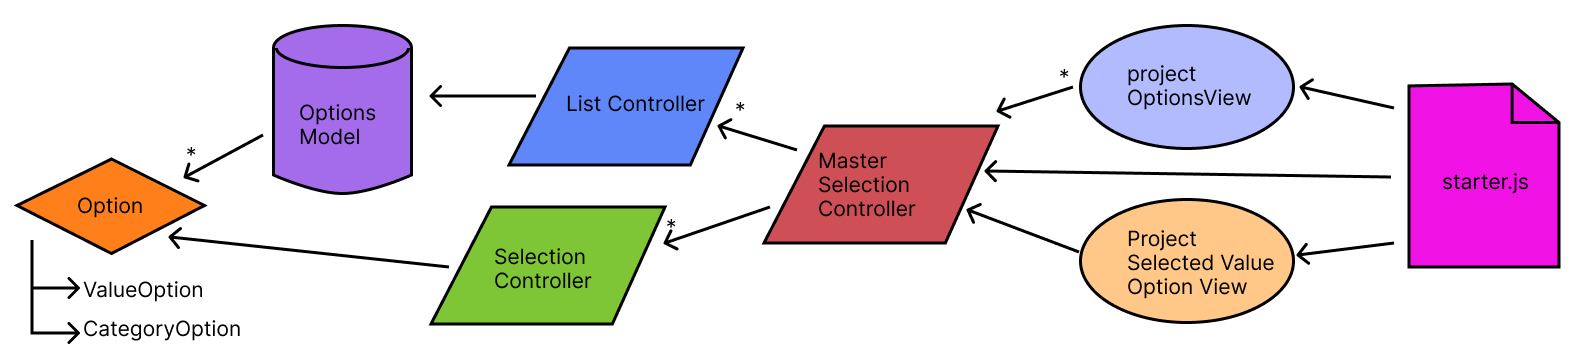
\includegraphics[width=120mm]{diagram-select-component-old.png}
    \caption{Diagramm Select Component - 1. Version}
    \label{Abbildung:DiagramSelectComponentOld}
\end{figure}

Der starter beinhaltet allte Bestandteile, welche für eine Anwendung benötigt werden.
Diese Version zeigte jedoch noch viel Komplexität und duplizierenden Code in den einzelnen Funktionen.
Nach einer genauen Analyse der Komponente war klas, dass sich das Pattern zwei Mal anwenden lässt.
Die neue Aufteilung ergibt die zwei folgenden Abbildungen \ref{Abbildung:DiagramColumnComponent} und \ref{Abbildung:DiagramSelectComponent}.
Die Implementation derer gaschah in einem Refactoring mit grösserem Rahmen.

\begin{figure}[!htb]
    \centering
    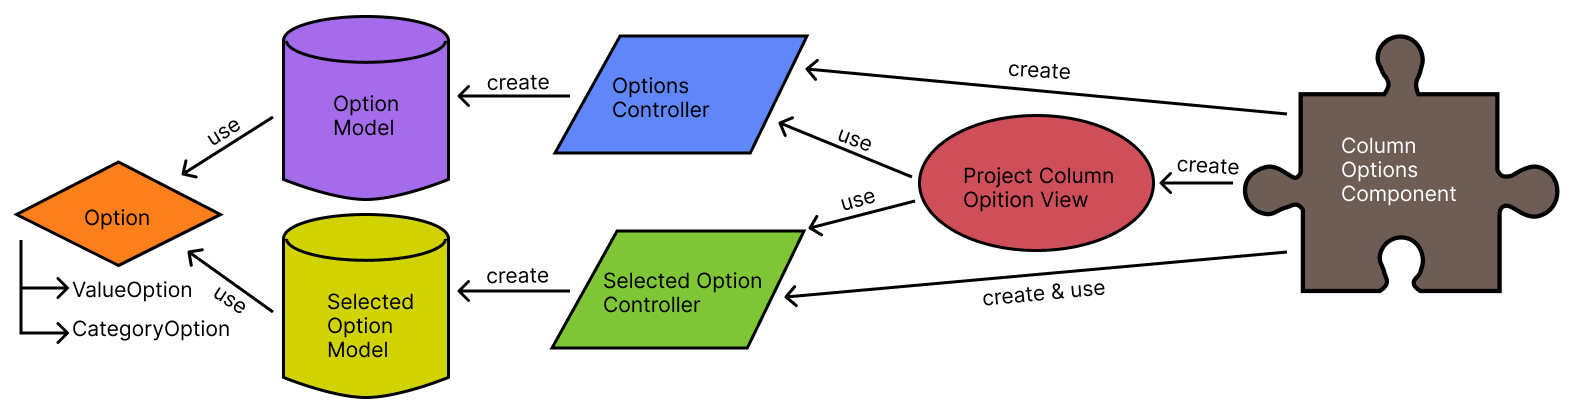
\includegraphics[width=120mm]{diagram-column-component-with-desc.png}
    \caption{Diagramm Column Component}
    \label{Abbildung:DiagramColumnComponent}
\end{figure}

Zum einen findet sich das Projector Pattern in einer einzelnen Spalte in der Options-Liste wieder.
Pro Kolonne exestiert eine Auswahl und eine Menge von Optionen.
Diese beiden Bestandteile besitzen je einen eigenes Model und ein eingenen Controller.
Der Projektor generiert in diesem Fall eine gemeinsame View mit Bindings zu den beiden Controller.
Die ColumnComponent verwaltet die Teile, welche eine Anwendung mit sich zieht (Mehr dazu später).

\begin{figure}[!htb]
    \centering
    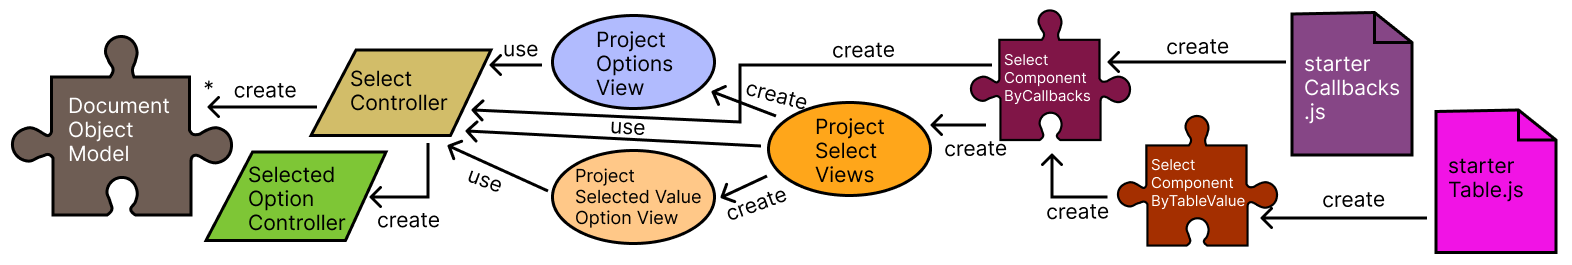
\includegraphics[width=120mm]{diagram-select-component-with-desc.png}
    \caption{Diagramm Select Component}
    \label{Abbildung:DiagramSelectComponent}
\end{figure}

Die Anwendungskomponete findet sich als Bestandteil des zweiten Projector Pattern wieder.
Ein SelectController verwaltet eine bis mehrere ColumnComponents als auch eine Cursor Position für die Tastaturnavigation.
Das Element für die Navigation verwendet im Hintergrund ebenfalls einen SelectedOptionController. 
Diese ist die selbe wie in der Abbildung \ref{Abbildung:DiagramColumnComponent} und findet hier eine Wiederverwendung.
Die Projektoren der einzelnen Teile greifen alle auf den selben Controller zu, um die Bindings zu definieren.
Der Master-Detail-Aufbau der neuen Komponente findet sich in der Aufteilung der Projektoren wieder.
Der Detail-Teil kümmert sich um die aktuellen Auswahl und das Eingabefeld.
Die Master-Komponete verwaltet alle Spalten mit den Kategorie- und Werte-Optionen, sowie dessen Bindings.
In einer weiteren Funktion werden die beiden Projektoren zusammengeführt und in eine gemeinsame View eingebettet.
Auch diese Projector Pattern Anwendung schliesst mit einer Component - der SelectComponent - ab.
Mehr zu dieser und der Column-Component steht im nächsten Kapitel.


\subsection{Decorator Pattern}

(\cite{decoratorPattern}) Ein Decorator bietet zusätzliches Verhalten ohne das Originale Objekt zu verändern.
Zudem können verschiedene Funktionen kombiniert werden.
Dieses Pattern ermöglicht eine modulare und anpassbare Software oder in diesem Projekt Auswahlkomponente zu gestalten.

Wie im vorherigen Kapitel erwähnt, besteht die neue Komponente unter anderem aus zwei sogenannten Component-Bausteinen.
Diese Bestandteile verwenden das Decorator Pattern in sofern, dass die Funktionalität des Controller mit der View kombiniert wird.
Dadurch kann die neue Kompnente einfacher angewendet werden.

\begin{lstlisting}[language = js, caption = SelectComponentByTableValue dekoriert SelectComponentByCallback, label = code:componentDecorator]
const SelectComponentByTableValues = (
    selectAttributes,
    optionsTable,
    sortColumnOptionsAlphabetical = false
) => {
    /* code for mapping between table and callbacks */
    const component = SelectComponentByCallbacks(selectAttributes, callbacks);
    return {
        ...component,
    };
};
\end{lstlisting}

Ein weiterer Einsatzort ist bereits in der Abbildung \ref{Abbildung:DiagramSelectComponent} aus dem Vorkapitel zu erahnen.
Der rotbraune SelectComponentByTableValue in Code \ref{code:componentDecorator} dekoriert die SelectComponentByCallback.
Damit bietet die neue Komponete zwei verschiedene Möglichkeiten der Anwendung.
Das nächste Kapitel geht noch genauer auf einen Teil des SelectProjectors aus Abbildung \ref{Abbildung:DiagramSelectComponent} ein.


\section{Dropdown-Container}

Um alle Options zu gegebender Zeit in geeigenter Form anzuzeigen anzeigen zu können.
Eine Möglichkeit ist, den Container als HTML-Dialog zu gestalten.
Die gebotenen Funktionen sind jedoch nicht auf die Anwendung dieser Komponente geeignet.
Für den gewünschten Zweck erfordert die Dialog-Komponente noch einige Anpassungen.

Ein normaler Div-Container als Options-Container zu verwenden, ist eine weitere Variante.
Dies erfordert ebenfalls einen enormen Implementationsaufwand.
In der ersten Version der Komponenten fand sich dieser Ansatz.
Hierbei zeigte sich das Problem, von der Inkonsistenz zwischen UI und Controller bzw. es konnten gleichzeitig mehrere Dropdown-Container offen sein.

Als dritte Möglichkeit bietet sich die Popover-API an, welche seit 2024 von allen gängigen Browser unterstützt wird.
In der neuen Version der Select-Komponenten findet sich diese Variante wieder.
Hier ist auch Zusatzaufwand notwendig, aber weniger als bei den beiden oben genannten Container-Implementationen.
Der Grundaufbau der Popover-Container ist im folgenden Code \ref{code:PopoverExample} dargestellt.

\begin{lstlisting}[language = html5, caption = Popover-Container Beispiel, label = code:PopoverExample]
<div popover="auto"
    id="select-component-0-options" 
    class="options-component" 
> </div>
\end{lstlisting}

Bei diesem Codeausschnitt ist wichtig, dass das Atttribut $popover$ den Wert $auto$ erhält.
Dies bewirkt, dass die Popover sich automatisch schliessen, wenn ein Klick ausserhalb des Container passiert.
Das Öffnen und Schliessen des Dropdown-Teil kann über das $popovertarget$-Attribut mit der Popover-Id auf der Bedienkomponente gesteuert werden.
Als Alternative dazu besteht die Möglichkeit, das Popover über JavaScript zu steuern.
Es kann ebenfalls auf den Status und das Event des Togglens zugegtriffen werden.
Durch diese Funktionalitäten ist der Controller konsistent mitführbar.


\section{Performance}

Um eine gute Performance zu bieten, ist es notwendig den Aufbau-Prozess einer Webseite zu kennen.
Dieser Ablauf ist im Kapitel \textbf{Grundalgen} unter \textbf{Ablauf Parsing \& Rendering} genau beschrieben.
Die folgende Abbildung \ref{Abbildung:RenderingProcessRecap} zeigt den Prozess im Überblick.

\begin{figure}[!htb]
    \centering
    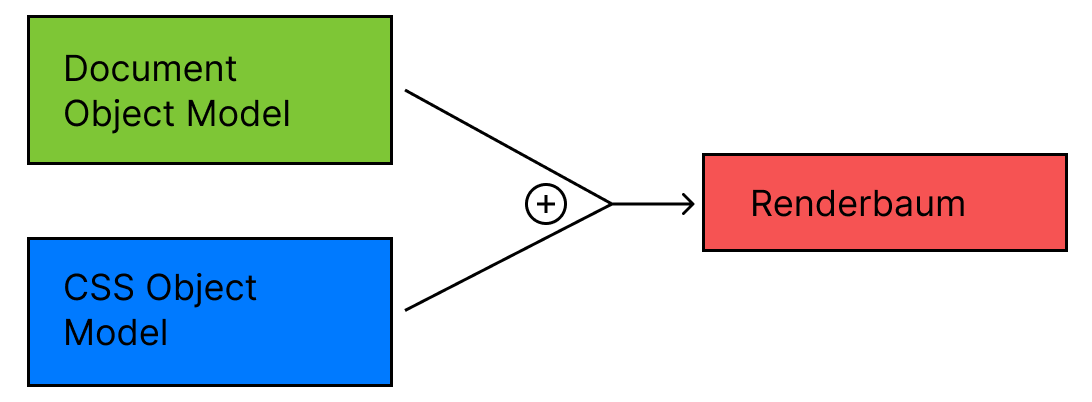
\includegraphics[width=120mm]{rendering-process.png}
    \caption{Rendering Prozess}
    \label{Abbildung:RenderingProcessRecap}
\end{figure}

Hierbei ist ein wichtiger Punkt, dass der Browser den Renderbaum (in der Abbildung \ref{Abbildung:RenderingProcessRecap} rot) maximal 60 Mal pro Sekunde neu zeichnen kann.
Daher müssen viele kleine Änderungen ausserhalb des Renderbaums - am besten in einem sogenannten Shadow-DOM - geschehen.
Ein Shadow-DOM ist ein Teilbaum, welcher nicht im Renderbaum angehängt ist.
Um dies zu bewerkstelligen, ist es sinnvoll, die Änderungen nach dem Abhängen des Elternknotens zu vollziehen. 
Nach den Änderungen kann der Teilbaum wieder an den gewünschten Ort platziert werden.

\begin{lstlisting}[language = js, caption = Performance Optimierung (columnOptionsComponent.js), label = code:PerformanceOptimization]
const addAllOptions = (options) => {
    const placeHolder = createHolder();
    columnView.replaceWith(placeHolder);
    if (options.length > 50) {
        setTimeout(() => {
            options.forEach((option) => {
                optionsController.addOption(option);
            });
            updateScrollbar(columnView);
            placeHolder.replaceWith(columnView);
        }, 80);
    } else {
        options.forEach((option) => {
            optionsController.addOption(option);
        });
        updateScrollbar(columnView);
        placeHolder.replaceWith(columnView);
    }
};
\end{lstlisting}

Code \ref{code:PerformanceOptimization} ist eine Stelle, die diese Technick verwendet.
Hier wird ein Platzhalter mit einem Lade-Indikator an die Ursprungstelle gesetzt, damit der Nutzer ein Feedback erhält.
Sobald der SpaltenContainer abgekoppelt ist, lädt die Funktion die Optionen in den Shadow-DOM.
Nach Abschluss wird der Container mit den neuen Elementen an die originale Stelle zurückersetzt.

(\cite{efficientDomManipulation}) Weiter ist darauf achten, dass CSS-Klassen an Stelle von Inline-Styles verwendet werden sollten.
Das Cachen von mehrfach verwendete Selektoren verbessert die Effizienz des DOMs.
Die Selektore sollten hierarchisch möglichst flach und nicht verschachtelt sein.
Zudem ist es, wenn es die Situation erlaubt, besser nicht mit innerHTML zu arbeiten.
In diesem Projekt ist es für die Anzeige der Label jedoch nötig innerHTML zu nutzen.
Dies liegt daran, dass ein Label auf ein Bild enthalten kann.
Der Inline-Style ist nur an einer Stelle in Gebrauch, damit die Properties nicht überschrieben werden können.

\begin{lstlisting}[language = html5, caption = Inline-Style für Inputfeld, label = code:InlineStyle]
inputElement.setAttribute(
    "style", "all: unset !important; z-index: -1 !important; " +
    "position: absolute !important; inset: 5px !important; " +
    "color: transparent !important; pointer-events: none !important;"
);
\end{lstlisting}

Diese Regeln in Code \ref{code:InlineStyle} sorgen dafür, dass das Eingabefeld transparent als auch zurückgesetzt.
Zudem ist das Input im Hintergrund und in der selben Grösse wie der Auswahlteil der Komponente ist.

\subsubsection{Performance Vergleich}

Durch die Anpassungen der Performance Optimierung, verbesserte sich die Ladezeit bei grossen Datenmenge enorm.
Die Testseite enthält 4 existierende und 4 neue Auswahlkomponenten mit den selben Inhalten wie je eines der Existierenden.
Je eine der Selects enthält eine grosse Datenmenge von über 4'000 Werten.
Die folgenden zwei Bilder zeigen die Messung während des Seitenaufbaus.

\begin{figure}[!htb]
    \centering
    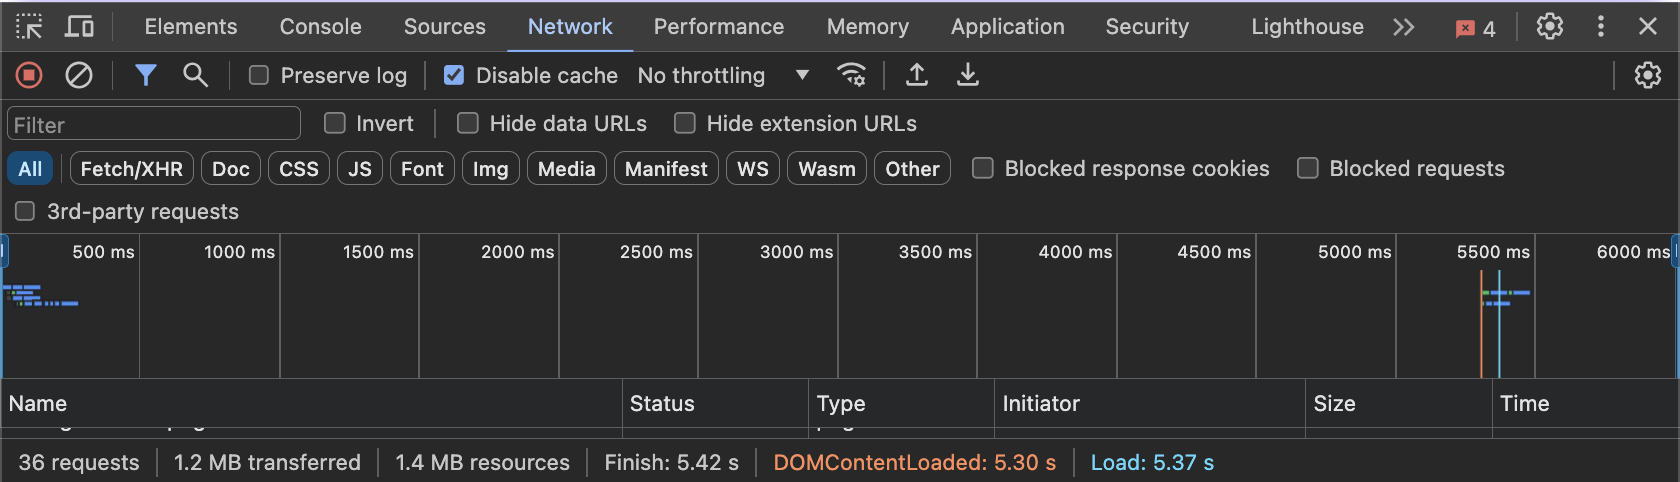
\includegraphics[width=100mm]{performance-before-user-tests.png}
    \caption{Performance Test vor Anpassungen}
    \label{Abbildung:PerformanceTestBefore}
\end{figure}

Auf der Grafik \ref{Abbildung:PerformanceTestBefore} ist zu sehen, dass der Seitenaufbau anfangs sehr lange dauerte.
Dies war auch ein Feedback der Nutzer, mehr dazu später.

\begin{figure}[!htb]
    \centering
    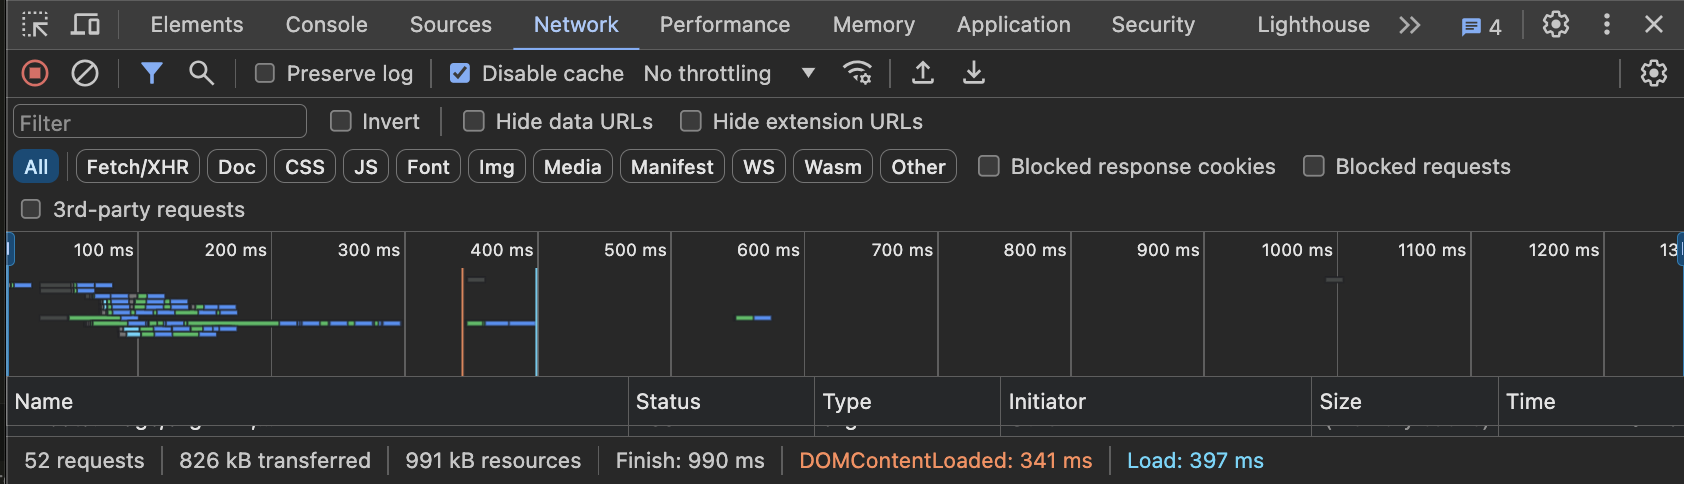
\includegraphics[width=100mm]{performance-after-user-tests.png}
    \caption{Performance Test nach Anpassungen}
    \label{Abbildung:PerformanceTestAfter}
\end{figure}

Der Vergleich zwischen Abbildung \ref{Abbildung:PerformanceTestBefore} und \ref{Abbildung:PerformanceTestAfter} zeigt, dass die Seite um einen Faktor 13 besser ist.
In der oberen Grafik wurden sehr viele Aktionen auf dem Renderbaum ausgeführt, welche durch ein Refactoring auf einen Shadow-DOM verschoben wurden.
Dadurch spart der Ladevorgang 4 bis 5 Sekunden an Wartezeit.
Im nachfolgenden Kapitel stehen Resultate und Feedbacks zu den durchgeführten User-Tests mit Programmierern als auch Endnutzern.


\section{User Tests}


\subsection{Programmierer}



\subsection{Formular-Ausfüller}



% Keyboard navigation. Using keyboard to narrow down possible categories/values (maybe fuzzy searching), otherwise it takes me longer to find something than compared to a standard dropdown, even if the list there is bigger.
% Teams Nachricht an Lea ;)
% ich finde es etwas unintuitiv beim SelectComponent neben den offensichtlich verständlichen selectAttriutes (labl, name, numberOfColumns) noch ein Callback mitzugeben.

% ich hätti mir mehr beschreibung gewünscht wie ich die komponente verwenden muss. (ich musste eher dannach suchen.
% Bessere Dokumentation war verwirrend (Code).
% - Doku: In der Code Doku von SelectComponent dürfte der Return Value besser beschrieben werden (welches Array Element ist was). Das wird erst in den Anwendungsbeispielen klar.
% - Detail: numberOfColumns ist etwas "verbose"
% Es würde helfen, wenn die Types im JSDOC spezifiziert wären und wenn die Library eingebunden wäre. Dann wäre die Dokumentation leichter auffindbar.
% War mir am Anfang nicht klar dass was SelectComponent() zurückgibt und ob das Input-element sowie dass label-element selbst erstellt werden soll. Danach war es intuitiv anzuwenden.

% ---------

% Nitpicking: while I see why the component is imported from a URL for the user tests, it makes it hard to use on a spotty network.
% ich persönlich hatte zu beginn schwierigkeiten zu verstehen wie das "framework" funktioniert. die beschreibung für die tasks (ab task2) sind zum teil etwas unklar =>

% The value data is provided by the function `Service.getRegionsByCountry()`,
% the categories are provided by the function `Service.getCountries()`

% RegionsByCountry muss man noch das Country mitgeben. Hätte in der beschreibung drinstehen können.

% ----------

%  Isch s selectAttributes `numberOfColumns` wörklich nötig? Ih be nämlich chli am umespiele gsii, met was passiert wenn mer `numberOfColumns` uuf en "falsche" Wert setzt oder eifach meh/weniger `serviceCallbacks` mit git. Vo mir uus gseh, chönt mer `numberOfColumns` vo  `serviceCallbacks.length` ableite...?
%  Ehr hend nah recht es performance Problem wenn d liste lang isch...Dur s implementiere vo Task 2.2 brucht d websiite ca. 5 sekunde zum lade (rein Javascript execution). Das liht ned ahm Javascript, sondern am HTML rendering sowiit ih gseh ha. Ha suscht nah e Performance Trace gmacht wo mer in Chrome chan drii lade ahhghänkt.
%  Isch betz speziell, dass `serviceCallbacks` array in vercherter reihefolg muen drii geh werde wies denne ahhzeigt wird...
%  Wenn mer 2 Kollone het, aber rechts ke uuswahl, de chan mer au nüt uuswähle... Ja isch z erwarte aber isch au ih de Demo vorhande
%  För mich isch ned immer klaar gsii, wenns nah meh optione unde oder obedraa het. Ih de Browser Dropdown liste gseht mer das sehr schnell dur pfiili obe und unde


\section{Diskussion}

% herausforderungen
% komplexeste probleme
% erfolge
% unerwartete wendungen
% entscheidungen, gründe => kein filter/ suche

\section{Fazit}
